\documentclass[14pt]{mmcs_article}
\usepackage[russian]{babel}
\usepackage{amsmath, amsthm, amsfonts, amssymb}
\usepackage{listings}
\usepackage{color}
\definecolor{lightgray}{rgb}{.9,.9,.9}
\definecolor{darkgray}{rgb}{.4,.4,.4}
\definecolor{purple}{rgb}{0.65, 0.12, 0.82}
\usepackage{csquotes}

%\graphicspath{{images/}}%путь к рисункам

\begin{document}


%см. РЕКОМЕНДАЦИИ ПО ОФОРМЛЕНИЮ
%И ПРЕДСТАВЛЕНИЮ КУРСОВЫХ И ВЫПУСКНЫХ %КВАЛИФИКАЦИОННЫХ РАБОТ СТУДЕНТОВ ИНСТИТУТА %МАТЕМАТИКИ, МЕХАНИКИ И КОМПЬЮТЕРНЫХ НАУК


% ----------------------------------
% Внимание!
% Изменяйте только строки, перед которыми стоят знаки комментариев
% ----------------------------------

\thispagestyle{empty}
\begin{singlespacing}
\begin{center}

МИНОБРНАУКИ РОССИИ\\ [12pt]
Федеральное государственное автономное образовательное\\
учреждение высшего образования\\
<<Южный федеральный университет>>

\vspace{\baselineskip}
Институт математики, механики\\
и компьютерных наук им.~И.\,И.~Воровича

\vspace{\baselineskip}
% Название выпускающей кафедры
Кафедра информатики и вычислительного эксперимента

\vfill
% Фамилия Имя Отчество студента
\textbf{Снегур Анастасия Тарасовна}

\vspace{\baselineskip}
%НАЗВАНИЕ РАБОТЫ должно полностью соответствовать
% приказу по ЮФУ (для выпускных квалификационных работ)
{\bf РАСПОЗНАВАНИЕ ИНФОРМАЦИИ \\
НА ИЗОБРАЖЕНИЯХ ЧЕКОВ ДЛЯ \\
ИСПОЛЬЗОВАНИЯ В КОРПОРАТИВНОЙ СИСТЕМЕ }

\vspace{15mm}
ВЫПУСКНАЯ КВАЛИФИКАЦИОННАЯ РАБОТА\\
по направлению подготовки\\
% Направление обучения
% раскомментируйте нужную строчку
%02.03.02~-- Фундаментальная информатика и информационные технологии
% 01.03.01~-- Математика
01.03.02~-- Прикладная математика и информатика
% 01.03.03~-- Механика и математическое моделирование 	


\vspace{10mm}
\textbf{Научный руководитель~--}\\
% указать данные о руководителе
% должность, степень, звание Фамилия Имя Отчество
Старший преподаватель Ячменёва Наталья Николаевна

\vspace{15mm}

\noindent
% указать Фамилию и инициалы 
% заведующего выпускающей кафедры
\begin{flushleft}
Допущено к защите:\\
заведующий кафедрой \underline{\hspace*{65mm}} Пилиди В.\,С.
\end{flushleft}




\vfill
% год!
Ростов-на-Дону -- 2020

\end{center}

\singlespacing
\end{singlespacing} % для работы бакалавра


\renewcommand{\contentsname}{Оглавление}

\tableofcontents

%=======================
\newpage
\addcontentsline{toc}{section}{Введение}
\section*{Введение} 
Процессы - это фундаментальная часть любого, будь то малого, среднего или крупного бизнеса. Они могут быть рассмотрены как алгоритмы, определяющие пути решения возникающих задач. При их построении, используется концепция BPM – Business Process Management – практика проектирования, выполнения, мониторинга и оптимизации бизнес-процессов.  Если рассматривать критерий автоматизации процессов более подробно, то необходимо обратиться к специальному программному обеспечению, которое поддерживает разработку технологических решений для выполнения бизнес-процессов. Одним из таких инструментов является Cloud Platform ServiceNow (SN) \cite{stud:b021}. 

Основное предложение ServiceNow — это готовая платформа, которая позволяет упростить и автоматизировать рутинные рабочие задачи и обеспечить плавное выполнение проектов с использованием единой модели данных. Сервис построен на инструментальной панели управления событиями (Event Management Dashboard), наглядно отображая состояние каждого элемента в различных сферах компании и предлагая быстрый доступ к оптимальным решениям. Это максимально абстрактное понятие включает возможность организовать любую необходимую работу, будь то обмен данными между сотрудниками, клиентская поддержка, ведение базы данных и документации. Гибкая система настроек помогает организовать работу для любого типа бизнеса, в любой среде, где есть доступ к интернету.
Ключевым фактором является то, что SN может стать отличным инструментом для конфигурации бизнес процессов, связанных с электронным документооборотом, так как обладает необходимыми для этого ресурсами:

\begin{itemize}
\item Централизованная организация документов в стандартизированных файловых структурах и форматах,
\item Защита документов в соответствии со список управления доступом,
\item Простота в распространении нужных документов среди работников,
\item Хранение и доступ к информации для более эффективного использования.
\end{itemize}

Но несмотря на полный спектр средств, направленных на автоматизацию и оптимизацию процессов связанных с документооборотом, актуальной остаётся проблема конвертации печатных документов в электронный формат.Именно поэтому в данной работе разработана система распознавания информации на изображениях кассовых чеков на основе возможностей платформы Service\-Now по внедрению преобразований бумажных документов в цифровые активы. Это облегчает и автоматизирует создание финансовой отчетности, так как пропадает необходимость вручную вносить в базу данных информацию о расходах сотрудников компании. Сотрудник сам загружает изображение чека в систему, на основе чего генерируются отчеты.
В качестве инструментов для распознавания данных были использованы  Google Vision AI API \cite{stud:b02} и JavaScript библиотека Tesseract.js \cite{stud:b01}.  Также для проверки правописания слов была подключена библиотека SpellChecker.js \cite{stud:b012}.


%=======================
\newpage
\addcontentsline{toc}{section}{Постановка задачи}
\section*{Постановка задачи}
Целью выпускной квалификационной работы является расширение базового функционала корпоративной ServiceNow платформы путём внедрения OCR инструментов для распознавания текста на изображениях кассовых чеков. В качестве таких инструментов были выбраны одни из самых популярных и пользующихся спросом сервисов:  Google Vision AI и Tesseract.JS. 

Можно выделить следующие этапы выполнения работы:
\begin{itemize}
\item Изучение особенностей и возможностей Cloud Platform ServiceNow,
\item Сбор и анализ тестовых данных,
\item Анализ существующих OCR сервисов и инструментов для распознавания текста на изображениях чеков,
\item Определение подходящего сервиса и изучение методов работы с API,
\item На основе проведённого анализа, внедрение Google Vision AI и \\Tesseract.js в ServiceNow,
\item Тестирование функционала конечного продукта,
\item Анализ полученных результатов.
\end{itemize}




%=======================
\newpage
\section{Обзор использованных в интеграции инструментов}\label{dsfs}
%=======================
\subsection{Особенности Cloud Platform ServiceNow}
ServiceNow - это полностью облачное решение, которое оптимизирует и согласовывает все внутренние процессы компании без необходимости приобретать или обслуживать дорогую инфраструктуру или дополнительное программное обеспечение. Многоэкземплярная архитектура лежит в основе работы платформы: для каждого сотрудника создается уникальный экземпляр (учётная запись в платформе), который поддерживает отдельный стек ресурсов. Это дает возможность реагировать на конкретные потребности каждого пользователя, что позволяет наладить работу на индивидуальной основе. 

Также стоит отметить, что в самой системе существует огромное количество "приложений" \- модулей, отвечающих за тот или иной бизнес-процесс. Например, существует модуль, который позволяет пользователю заказать новое оборудование или создать инцидент. Эти приложения представляют собой таблицы со своей уникальной структурой и логикой. Пользователи с правами системного администратора могут ограничивать доступ, вносить изменения в логику и структуру приложений, конфигурировать таблицы и записи.
%=======================
\subsubsection{Некоторые понятия, использованные в работе}
Триггер -  хранимая процедура особого типа, которую пользователь не вызывает непосредственно, а исполнение которой обусловлено действием по модификации данных.
REST Message используют протоколы HTTP в качестве средства связи между клиентом и сервером. Клиент отправляет сообщение в форме HTTP-запроса, а сервер отвечает в виде HTTP-ответа.
REST API - то общие принципы организации взаимодействия приложения/сайта с сервером посредством протокола HTTP. 
KPI (Key Performance Indicator) — это показатель достижения успеха в определенной деятельности или в достижении определенных целей.
OCR (optical character recognition) - это технология, позволяющая преобразовывать различные типы документов,  в редактируемые форматы. Например изображение с текстом в текстовый формат.
SDK - набор средств разработки, который позволяет специалистам по программному обеспечению создавать приложения.
AI - искусственный интеллект.
%=======================
\subsubsection{Приложения SN, задействованные в разработке} 
\begin{itemize}
\item Business Rules (BR) \cite{stud:b1} представлены в виде серверного кода, который запускается, когда запись из таблицы отображается/вставляется/обновляется/удаляется, а также когда запрашивается непосредственно сама таблица. В основном BR принято использовать для выполнения таких задач, как автоматические изменения значений в полях формы при соблюдении определенных условий. Возможно настроить отправку всевозможных уведомлений. В интеграции используется для отправки REST запроса, получения ответа от сервера в виде JSON объекта и дальнейшей работы с ним. Триггером служит добавление изображения на форму.
\item Script Includes \cite{stud:b2} используются для хранения JavaScript кода, который действует на сервере платформы. Каждая запись данного модуля хранит функции и классы для глобального использования. Алгоритмы кодирования изображения в формат BASE64 и формирование тела JSON запроса было решено вынести в Script Include отдельным классом. Этот шаг предоставил возможность облегчить читаемость созданного BR кода.
\item REST (Representational State Transfer) \cite{stud:b3} представляет собой архитектуру, обеспечивающую связь между компьютерными системами в Интернете, облегчая для них взаимодействие друг с другом. Платформа Now предоставляет различные REST API, которые по умолчанию активны. Эти API предоставляют возможность взаимодействия с различными функциями ServiceNow в вашем приложении. Такая функциональность включает в себя возможность выполнения операций создания/чтения/обновления/удаления в существующих таблицах, вставки данных, извлечения информации и запуска преобразований для базы данных.
\item Client Scripts \cite{stud:b4} позволяют системе запускать JavaScript код на клиентской стороне (веб-браузере), когда форма загружается, поле меняет значение, или когда изменения на форме сохраняются. С помощью данного модуля реализована интеграция с библиотекой \\ Tesseract.js.
\item Service Portal \cite{stud:b5} — один из многочисленных модулей ServiceNow, позволяющий разработчикам и администраторам создавать действительно удобный пользовательский интерфейс, с интуитивно понятным управлением. Он взаимодействует с существующими компонентами ServiceNow, поэтому пользователи могут получать доступ к определенным функциям платформы с помощью него, например воспользоваться виджетами для распознавания текста.
\item UI Scripts \cite{stud:b6} предоставляют возможность не только хранить клиентский JavaScript, но и запускать его «из браузера», встраивать в HTML код страницы. Принцип работы схож с «Script Includes», только применяется не для серверной, а для клиентской части. В рамках поставленной задачи, используется для хранения библиотек Tesseract.js и Spell-checker.js.
\item UI Pages \cite{stud:b7} могут использоваться для создания и отображения форм, диалоговых окон, списков и других компонентов пользовательского интерфейса.
\item Performance Analytics \cite{stud:b8} - это платформенное решение для оптимизации процессов, позволяющее создавать информационные панели управления, составлять отчеты по KPI и метрикам, а также отвечать на ключевые бизнес-вопросы, помогая повысить качество и сократить расходы на предоставление услуг,
\item System Properties \cite{stud:b9} модуль задействован для того, чтобы скрыть в коде уникальные ключи записей, пароли и другую конфиденциальную информацию, 
\item UI Action \cite{stud:b10} включают кнопки, ссылки и элементы контекстного меню в формах и списках, чтобы сделать пользовательский интерфейс более интерактивным.
\end{itemize}
%=======================
\subsubsection{Преимущества использования данного облачного сервиса}
\begin{itemize}
\item Платформа позволяет разрабатывать с использованием новейших веб-технологий и поддерживает интеграцию со сторонними приложениями. Служба поддержки клиентов ServiceNow эффективно решает любые вопросы/заявки.
\item Для того, чтобы иметь доступ к личному экземпляру платформы, необходимо лишь создать учётную запись на официальном портале.
\item ServiceNow отлично справляется с большинством административных обязанностей, включающих в себя документирование и организацию проектных задач, обеспечивая своевременную связь и соблюдение всех нюансов и тонкостей. Данное преимущество позволяет автоматизировать рутинные бизнес-процессы (создание запросов, отчётов, ведение учёта времени) и тем самым сохранить время для по-настоящему важных дел, например для создания итогового продукта,
\item Подробная техническая документация доступна на официальном сайте.
\end{itemize}

%=======================
\subsection{Анализ и классификация чеков}
Федеральным законом РФ установлено два вида платёжных документов: обычный (на бумажной кассовой ленте) и электронный. Первый выдаётся при принятии оплаты в торговом пункте, второй направляется через SMS-сообщение или на e-mail при любой онлайн покупке. В данной работе рассмотрены оба типа кассовых чеков, так как принципы распознавания каждого из них одинаковы. Каждый чек должен включать в себя следующие реквизиты:
\begin{itemize}
\item Наименование организации либо ИП,
\item Сумма, на которую пробит чек,
\item Дата и время транзакции,
\item Номер документа (чека),
\item Номер кассового аппарата,
\item Номер ЭКЛЗ,
\item Номер КПК по порядку,
\item значение КПК - контрольный проверочный код.
\end{itemize}

На изображении (рис.\,\ref{stud:fig:01}) красным отмечена ключевая информация, которая в последующем будет храниться в виде записей в самой платформе. Зелёный указывает на необязательные, но также полезные данные. 
\begin{figure}[H]
  \centering
  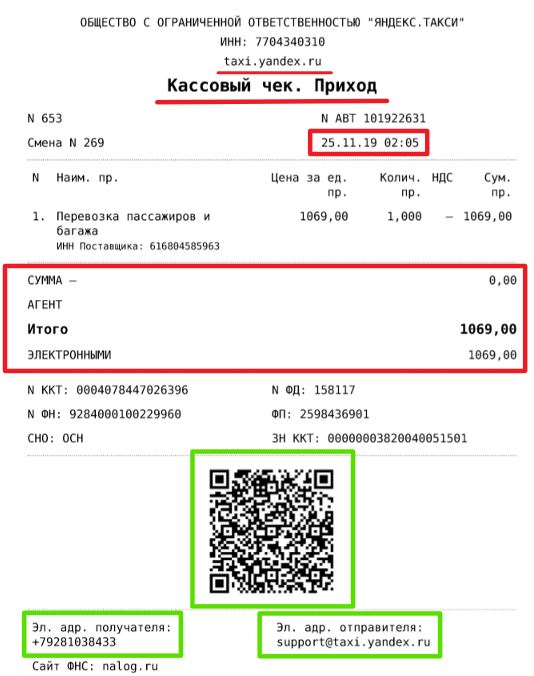
\includegraphics[scale=0.5]{boxes.JPG}
  \caption{Важные реквизиты кассового чека}\label{stud:fig:01}
\end{figure}
Проанализировав данные о покупках товаров и услуг, совершаемых внутри компаний, можно выделить основные типы, пользующиеся спросом (рис.\,\ref{stud:fig:101}). Для каждого из них характерен определённый словарный состав. Проверив документ на наличие слов, подтверждающих принадлежность к тому или иному типу, можно сделать вывод и о самом классе денежной транзакции. Например, если в кассовом чеке встречаются названия продуктов питания, то логично будет заключить, что данные расходы можно определить в категорию "Питание".
\begin{figure}[H]
  \centering
  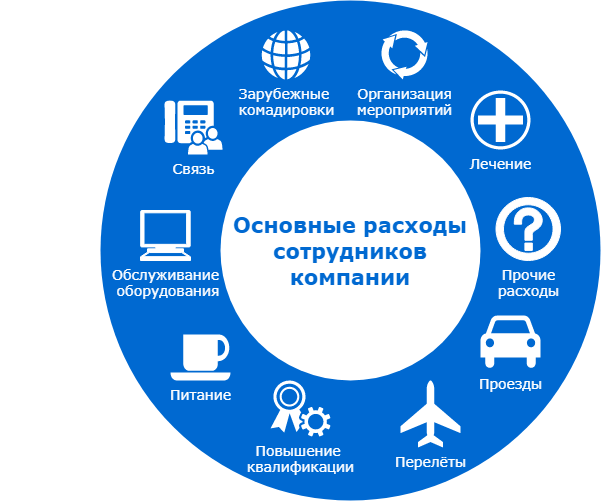
\includegraphics[scale=0.5]{dia.png}
  \caption{Классификация расходов}\label{stud:fig:101}
\end{figure}
%=======================
\subsection{Анализ существующих OCR сервисов}
OCR (optical character recognition) расшифровывается как «Оптическое распознавание символов». Это процесс преобразования изображения в машинный код. Например, мы можем получить отсканированное изображение книги и использовать технологию распознавания текста, чтобы прочитать изображение и вывести текст в формате, который мы можем использовать на любом вычислительном устройстве.

Критерии, по которым оценивались предложенные на рассмотрение сервисы:
\begin{itemize}
\item Качество распознанного текста,
\item Экономическая обоснованность,
\item Возможность интегрирования в платформу,
\item Распознавание текста, включающего в себя более одного языка.
\end{itemize}

Для получения более наглядных результатов, сервисам было предложено справиться с данным тестовым изображением (рис.\,\ref{stud:fig:1}).
\begin{figure}[H]
  \centering
  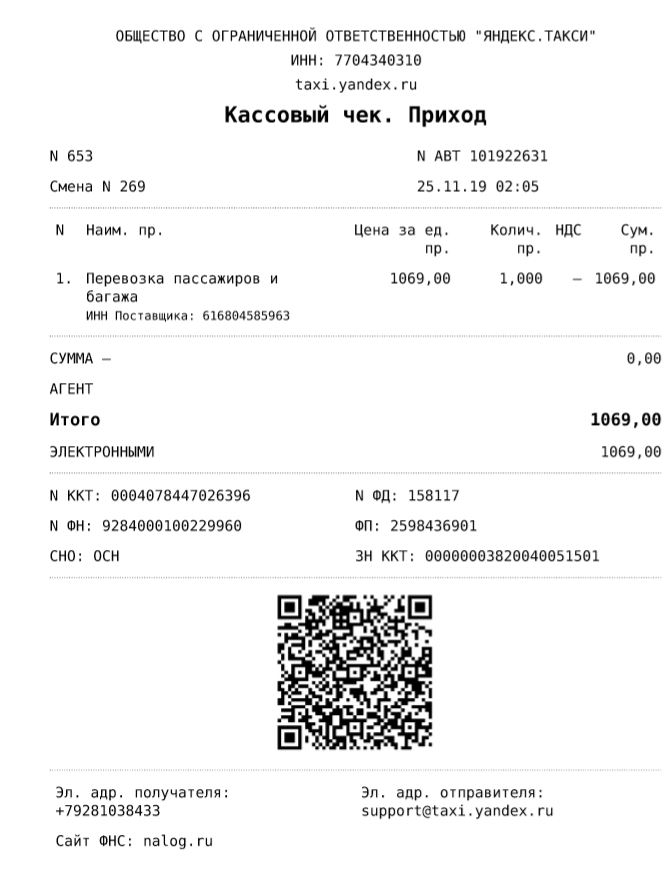
\includegraphics[scale=0.5]{Снимок.JPG}
  \caption{Изображение кассового чека}\label{stud:fig:1}
\end{figure}
\subsubsection{Tesseract JS}

Tesseract.js - JavaScript библиотека для распознавания текста на изображениях, поддерживающая огромное количество языков, включая русский и английский языки.

Текст полученный, в результате использования Tesseract.js (рис.\,\ref{stud:fig:2}).

\begin{figure}[H]
  \centering
  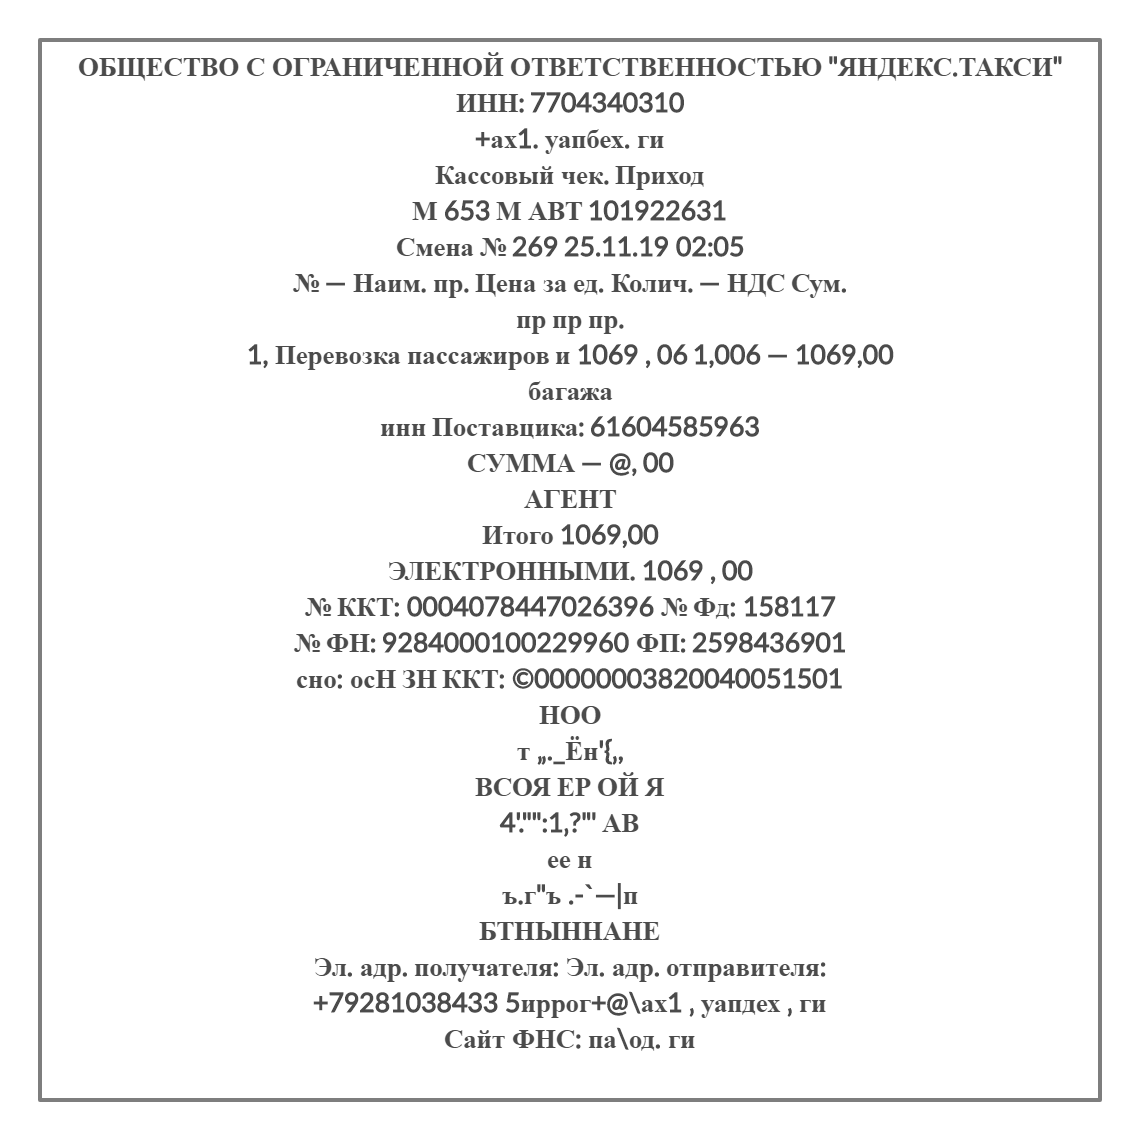
\includegraphics[scale=0.35]{test1.png}
  \caption{Tesseract.js}\label{stud:fig:2}
\end{figure}
\noindentДостоинства:
\begin{itemize}
\item Автоматическая ориентация текста,
\item Открытый код,
\item Бесплатное использование,
\item Доступный интерфейс для определения пространственных границ слов, абзацев,
\item Может работать как в браузере, так и на сервере с NodeJS.
\end{itemize}
Недостатки:
\begin{itemize}
\item Невозможность распознавания текста, включающего в себя более одного языка,
\item Зашумлённый фон и нестандартные шрифты существенно снижают точность обработки,
\item Ограниченный спектр возможностей.
\end{itemize}
Вывод:

На первый взгляд, данная библиотека является лучшим решением для распознавания чеков, так как возможность запускать скрипты на клиентской стороне является выигрышной при интеграции с платформой SN. Также стоит отметить, что с экономической точки зрения выгодно использовать этот инструмент, потому что он не требует дополнительных вложений (например приобретения подписки). Но несмотря на превалирующие достоинства, неспособность распознавать более одного языка одновременно препятствует получению хорошего результата.

\subsubsection{ABBYY Cloud OCR FineReader Engine} 
 
ABBYY FineReader Engine – многофункциональный инструментарий разработчика, который позволяет встраивать в приложения интеллектуальные технологии распознавания данных. С помощью OCR на основе технологий искусственного интеллекта вы можете создавать приложения с функциями качественного распознавания информации из документов, изображений, фотографий, скриншотов, мониторов и дисплеев, определения типа документа, конвертации сканированных документов в файлы форматов Word, Excel и PDF с возможностью поиска.

Текст полученный, в результате использования FineReader Engine (рис.\,\ref{stud:fig:3}).
\begin{figure}[H]
  \centering
  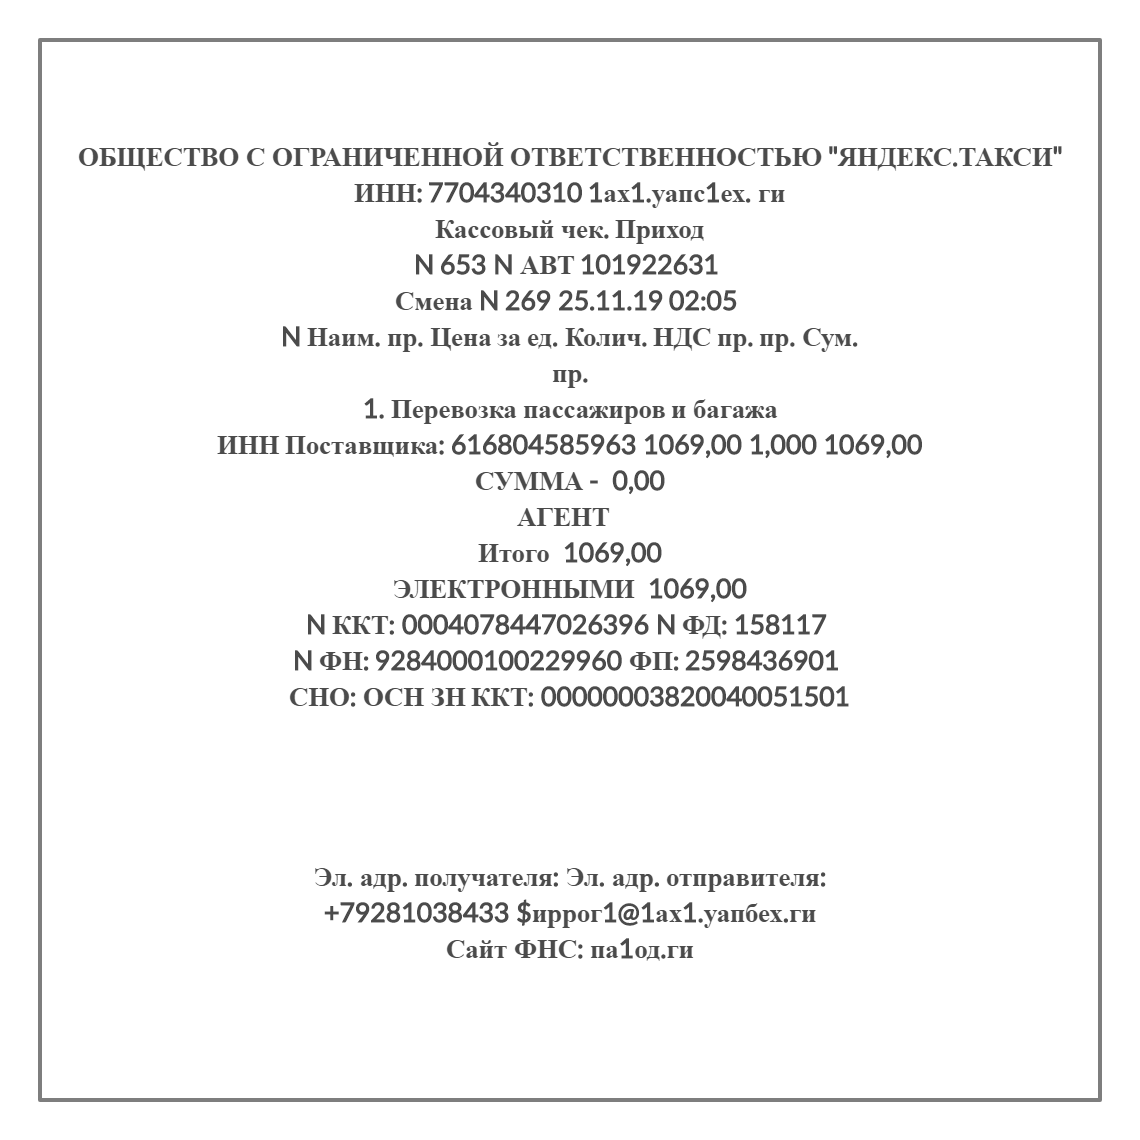
\includegraphics[scale=0.35]{test3.png}
  \caption{FineReader Engine}\label{stud:fig:3}
\end{figure}
\noindentДостоинства:
\begin{itemize}
\item Высокая точность распознавания,
\item Полный спектр технологий распознавания,
\item Инструменты для обработки PDF,
\item Поддержка множества языков,
\item Распознавание текста, включающего в себя более одного языка.
\end{itemize}
Недостатки:
\begin{itemize}
\item Высокая стоимость подписки.
\end{itemize}
Вывод:

 Данный сервис показывает высокое качество распознанного текста. Также стоит отметить удобство при работе с интеграцией: клиентская программа, передавая изображения с помощью одного или нескольких POST-запросов, формирует задание на сервере. После того, как задание сформировано, необходимо отправить его на обработку, указав настройки обработки. Кроме того, автоматическое определение языка позволяет сервису распознавать разноязычный текст, что делает его выигрышным по сравнению с Tesseract.js. Единственным недостатком становится ощутимая плата за использование данного инструмента, что делает его выбор экономически нерациональным.
 
\subsubsection{Google Vision AI}  
 
API Google Cloud Vision позволяет разработчикам легко интегрировать функции обнаружения объектов в приложение. Мощные, предварительно обученные модели машинного обучения достойно справляются с такими задачами, как распознавание лиц и ориентиров, оптическое распознавание символов (OCR), классификация изображений по множественным категориям.

Текст полученный, в результате использования Google Vision AI(рис.\,\ref{stud:fig:4}).
\begin{figure}[H]
  \centering
  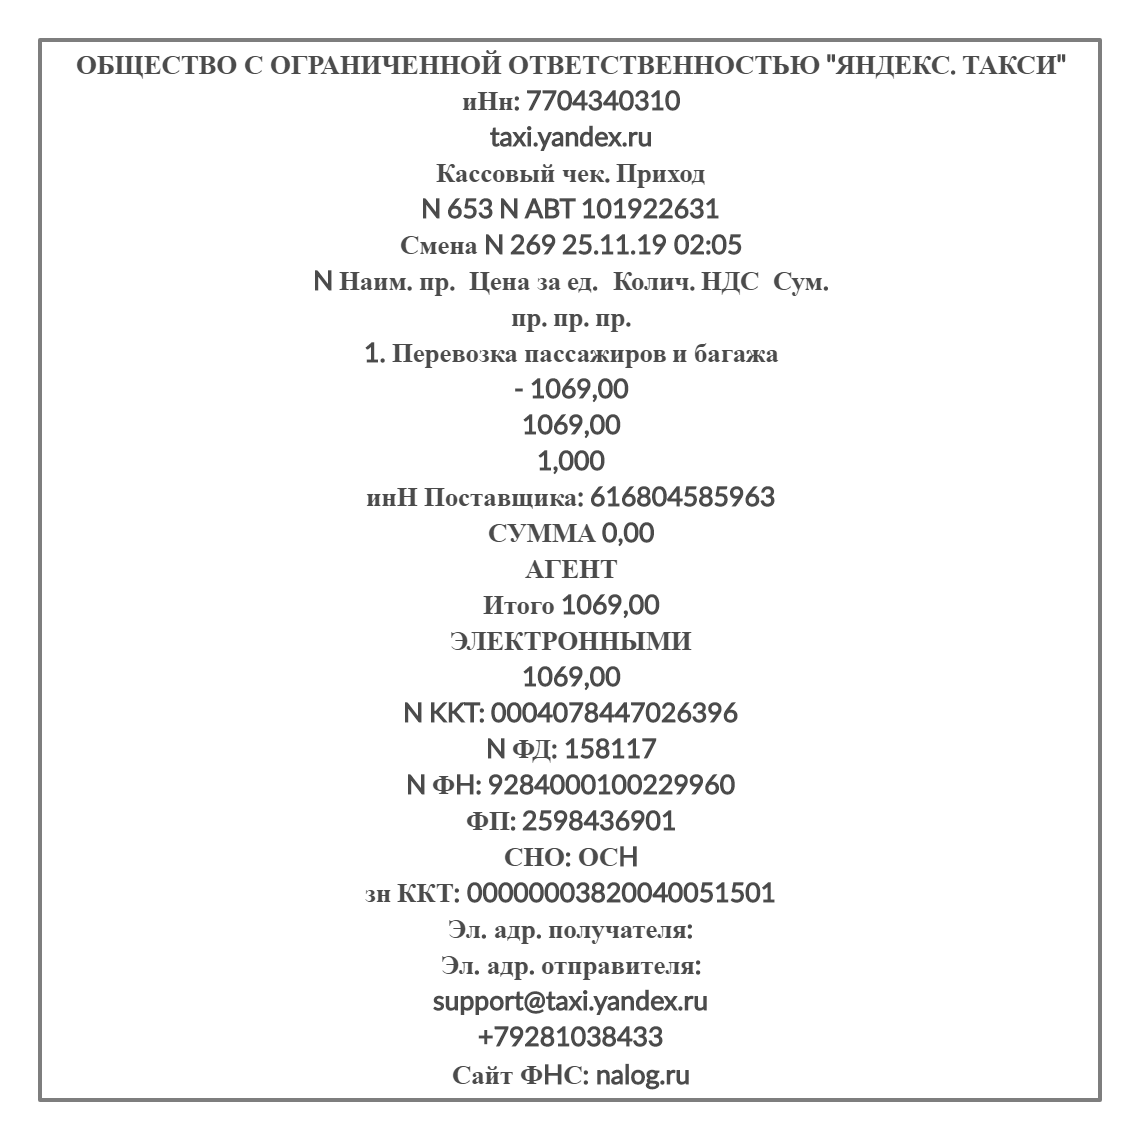
\includegraphics[scale=0.35]{test2.png}
  \caption{Google Vision AI}\label{stud:fig:4}
\end{figure}
\noindentДостоинства:
\begin{itemize}
\item Высокая точность распознавания,
\item Простота использования,
\item Распознавание текста, включающего в себя более одного языка,
\item Бесплатное использование на протяжении года,
\item Поддержка множества языков.
\end{itemize}
Недостатки:
\begin{itemize}
\item Ограниченное количество бесплатных запросов в месяц.
\end{itemize}
Вывод:

Google Vision AI обладает всеми преимуществами рассмотренного ранее ABBYY Cloud OCR SDK сервиса. Тестовые прогоны картинок показали сопоставимые результаты. Также схожи принципы передачи изображения для последующего рассмотрения с помощью POST-запросов. Главным достоинством данного инструмента является возможность на протяжении года использовать сервис без каких-либо денежных вложений, но с ограниченным количеством запросов в месяц. Поэтому было принято решение использовать данный сервис для поставленных задач.


%=======================

\section{Реализация распознавания информации на изображениях чеков}

%=======================
\subsection{Внедрение Google Vision AI в корпоративную систему}
\subsubsection{Подготовительный этап}
Чтобы использовать API, необходимо воспроизвести следующие шаги в Google Cloud Developer Console:
\begin{itemize}
\item Создать проект в Google Cloud Console или использовать уже существующий,
\item Включить в проекте Billing. Если это первое использование Google Cloud Console, необходимо начать бесплатный пробный период использования. Будут запрошены данные карты, но денежные средства будут списывать только в случае превышения лимита запросов,
\item Активировать Google Cloud Vision API,
\item B меню консоли необходимо перейти в Диспетчер API, затем в раздел "Учетные данные" \ и создать ключ API, который будет использоваться для формирования endpoint url.
\end{itemize}

Данная блок-схема (рис.\,\ref{stud:fig:10}) наглядно демонстрирует процесс получения текста, содержащегося в изображении. 
\begin{figure}[H]
  \centering
  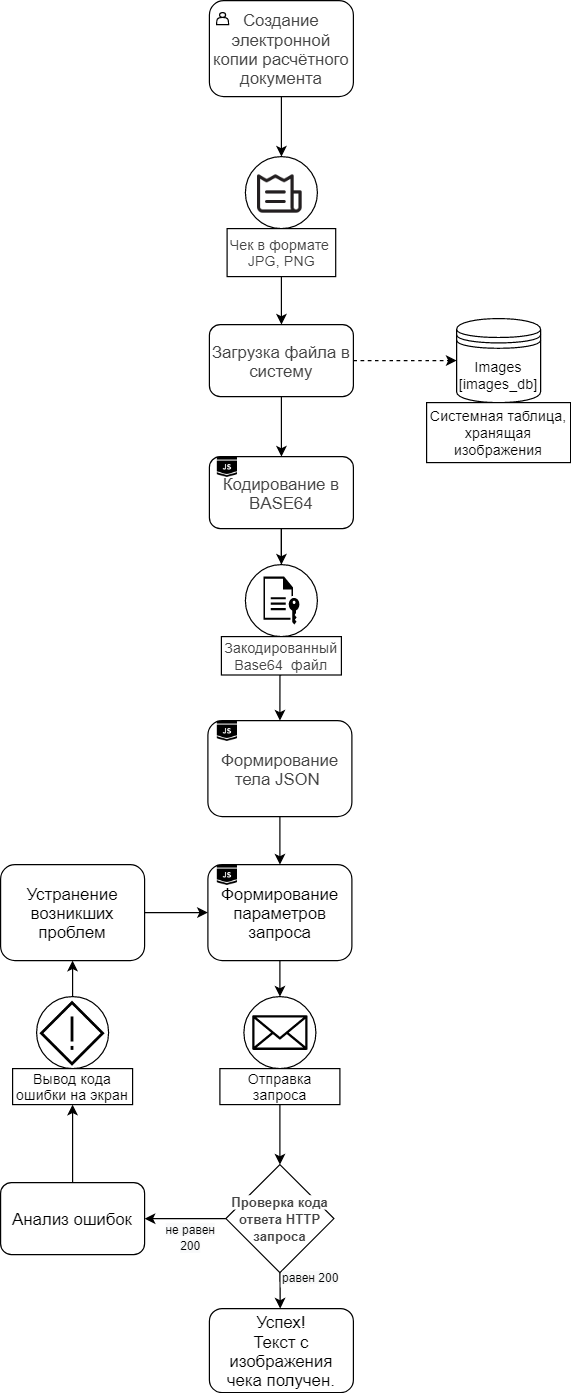
\includegraphics[scale=0.5]{GAI.png}
  \caption{Распознавание чеков с помощью Google Vision AI}\label{stud:fig:10}
\end{figure}
Рассмотрим некоторые этапы более подробно.
\subsubsection{Кодирование изображение в Base64 формат}
 Кодирование Base64 вводит избыточность, увеличивая размер. Основная цель - сделать так, чтобы данные могли быть представлены исключительно в виде текста. Есть ряд ситуаций, для которых шифрование необходимо. Например, в интеграции, для того чтобы защитить файлы от кражи (к чему могло бы привести открытие публичного доступа), было принято решение передавать закодированное изображение. Наиболее примечательным является то, что форматы сообщений для электронной почты раньше не принимали двоичный код. Кодировка Base64 преобразует файл так, что он содержит только буквенно-цифровые символы без знаков препинания (за исключением, возможно, одного или двух знаков равенства в конце). Это позволяет поместить его как текст электронного письма (или в любом другом контексте, где текст разрешен) и отправить его так, чтобы его можно было восстановить на другой стороне. Это не единственный способ передать файл в закодированном виде. Очевидно, можно просто кодировать как текст, запоминая шестнадцатеричное значение каждого байта. Это означало бы, что каждый байт в исходных данных становится двумя символами в кодировке, то есть удваивается размер данных. Base64 кодирует каждые три байта ввода, используя четыре байта на выходе. Вместо того, чтобы удваивать размер, он только увеличивает его на треть. Он добавляет некоторую избыточность, но не такую существенную, и позволяет восстанавливать данные при передаче по каналу, который разрешает только текст.

С целью закодировать документ была создана функция (Листинг \ref{stud-lst:5}.), основанная на методе base64Encode() встроенной библиотеки GlideStringUtil. Функция получает разбитое на биты методом getBytes() изображение. Для того чтобы получить доступ к нему, необходимо прописать запрос к таблице [sys\_attachment], хранящей все существующие в системе документы (изображения в том числе). Первичный ключ, присвоенный изображению, передаётся в качестве параметра запроса.
\begin{lstlisting}[caption=Base64 кодирование, label=stud-lst:5]
 base64Encode: function(attachID) {
        var AttachGR = new GlideRecord('sys_attachment');
        AttachGR.addQuery('table_sys_id', attachID);
        AttachGR.query();
        var base64 = '';

        if (AttachGR.next()) {
            var sysAttach = new GlideSysAttachment();
            var binData = sysAttach.getBytes(AttachGR);
            base64 += GlideStringUtil.base64Encode(binData);
            return (base64);
        }
    },
\end{lstlisting}
\subsubsection{Формирование JSON Request}
Согласно официальной документации, сервис должен получить JSON объект с полями:
\begin{itemize}
\item requests (представляет собой массив, состоящий из объектов, описанных ниже),
\item image (объект с полем content, где содержится Base64 закодированное изображение),
\item features (массив с указанием нужного типа распознавания type, в данном случае TEXT\_DETECTION).
\end{itemize}

Для формирования запроса (Листинг \ref{stud-lst:41}.) необходимо передать функции закодированное ранее изображение, затем создать строковую переменную, поместив в неё структуру будущего JSON объекта. Далее необходимо преобразовать переменную obj в JSON формат с помощью встроенного в систему метода encode. Функция возвращает готовое к отправке на сервер тело HTTP запроса. 
\newpage
\begin{lstlisting}[caption=Функция создания JSON запроса, label=stud-lst:41]
 requestJSON: function(b64Image) {
        var obj = {
            "requests": [{
                "image": {
                    "content": b64Image
                },
                "features": [{
                    "type": "TEXT_DETECTION"
                }]
            }]
        };

        var parser = new JSON();
        var request = parser.encode(obj);
        return (request);
\end{lstlisting}
 

\subsubsection{Отправка Rest Message}
REST API ServiceNow позволяет извлекать/создавать/обновлять/удалять данные на сервере веб-служб, которые поддерживают REST архитектуру.
Для того чтобы отправить запрос (Листинг \ref{stud-lst:041}.) на Cloud Google сервер, необходимо обратиться к встроенным в платформу методам \\RESTMessageV2(). Сначала необходимо указать, что это POST HTTP запрос, добавить url конечной точки связи (должен включать в себя ранее созданный в Google Cloud Console ключ). Передаём данные для базовой HTTP авторизации. Остаётся только описать тело запроса и запрос готов к отправке.     
\begin{lstlisting}[caption=Rest Message, label=stud-lst:041]
        var restMessage = new sn_ws.RESTMessageV2();
        restMessage.setHttpMethod("POST");
        restMessage.setEndpoint(gs.getProperty('google.auth.endpoint'));
        restMessage.setBasicAuth(username, password);
        restMessage.setRequestBody(reqBody);
        var response = restMessage.execute();

\end{lstlisting}

\subsubsection{Обработка JSON Response}
Получив ответ от сервера, необходимо удостовериться, что код статуса ответа находится в пределах от 200 до 299. Именно этот числовой промежуток характеризует был ли успешно выполнен определённый HTTP запрос. В случае, когда все условия соблюдены, необходимо получить тело ответа в виде JSON объекта, воспользоваться методом JSON.parse(). Далее следует полю [u\_vision] на форме присвоить текстовое значение, хранящееся по данному адресу указанному в 4 строке (Листинг \ref{stud-lst:6}.). Если же случилась проблема в процессе отправки запроса или получения ответа, необходимо вывести сообщение об ошибке (строки 6-10).
\begin{lstlisting}[caption=JSON Request, label=stud-lst:6]
       if (response.getStatusCode() === 200) {
            var responseBody = response.getBody();
            var responseData = JSON.parse(responseBody);
            current.u_vision = responseData.responses[0].fullTextAnnotation.text;
            current.update();
        } else {
            // process error response
            var statusCode = response.getStatusCode();
            var erorMessage = response.getErrorMessage();
            var contentType = response.getHeader("Content-Type");
            var body = response.getBody();
        }
\end{lstlisting}
%=======================
\subsubsection{Создание модального окна}
Для дальнейшей работы с распознанным текстом необходимо сконструировать дополнительное модальное окно (рис.\,\ref{stud:fig:123}) в интерфейсе Service\-Now. Основная задача этого элемента по ключевым словам заполнить поля будущей записи в системной таблице расходов компании, а затем создать её.
\begin{figure}[H]
  \centering
  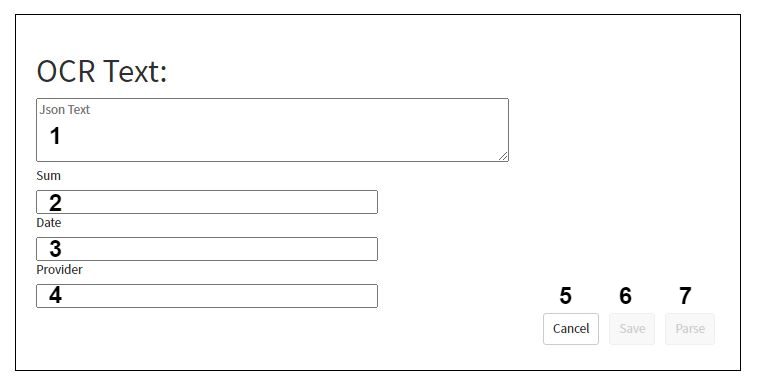
\includegraphics[scale=0.5]{UI Page.png}
  \caption{Форма для обработки распознанного текста}\label{stud:fig:123}
\end{figure}
Текстовое поле номер 1 предназначено для того, чтобы получить содержимое чека и исключить все орфографические ошибки, допущенные при распознавании. Для проверки орфографии используется встраиваемая JS библиотека Spell-checker.js. Так же поле намеренно было оставлено редактируемым, для того чтобы у пользователя была возможность вручную подправить огрехи. 

Далее следует нажать кнопку Parse (номер 7 на изображении), чтобы поля 2-4 заполнились в соответствии с их названиями. С помощью встроенного метода indexOf() происходит поиск необходимой информации по ключевым словам, которая затем будет передана каждому из полей. Если пользователя устраивает итоговая заполненная форма, он может с помощью клавиши Save (6) сохранить результат в виде записи в таблице расходов, а по нажатию клавиши Cancel, все предыдущие действия будут отменены.

%=======================
\subsection{Внедрение Tesseract JS в корпоративную систему}
В ситуациях, когда невозможно получить ответ от облачного сервера Google, необходимо предусмотреть существование запасного варианта, не зависящего от стабильности работы сторонних API. Таким вариантом как раз является библиотека Tesseract.js, хранящаяся локально в UI Script записях SN. Несмотря на то, что качество распознанного текста не сопоставимо с качеством, которое показывает Vision AI, после обработки и некоторых правок сделанных вручную в модальном окне, можно достичь желаемого результата.
Во время работы с данной библиотекой были воспроизведены следующие шаги:
\begin{itemize}
\item Локальное добавления библиотеки Tesseract.js

Для того чтобы использовать возможности JS библиотеки внутри ServiceNow платформы, необходимо:
    \begin{itemize}
    \item Выгрузить файл с исходным кодом библиотеки, перейдя по указанной ссылке \cite{stud:b01}
    \item Создать глобальную запись "OCR.jsdbx"\ в модуле UI Script
    \item В запись добавить исходный код из скачанного ранее файла
    \end{itemize}
\item Конфигурация и настройка системной таблицы Images [db\_images] (добавление недостающих полей на форму),
\item Создание Client Script (Листинг \ref{stud-lst:1}.),
\item Отображение итогового результата на форме.
\end{itemize}
Так как клиентский скрипт  срабатывает по изменению значения в поле OCR language, задаём OnChange функцию, которая отслеживает эти изменения. С помощью метода getScripts подключаем библиотеку. В метод recognize передаём:
        \begin{itemize}
        \item Ссылку изображения, которая состоит из неизменяемой части\\   "https://dev103823.service-now.com/"\ (адрес личного экземпляра\\ платформы) и непосредственно названия изображения,
        \item Язык (передаётся в переменную newValue, когда пользователь выбирает значение в поле "OCR language"),
        \item Объект настроек с логгером.
        \end{itemize}
        \newpage
\begin{lstlisting}[caption=Распознавание чеков с помощью Tesseract.js, label=stud-lst:1]
function onChange(control, oldValue, newValue, isLoading, isTemplate) {
   if (isLoading || newValue === '') {
      return;
   }

    ScriptLoader.getScripts('OCR.jsdbx', function() {
        Tesseract.recognize('https://dev10382.service-now.com/' + g_form.getValue('name'), newValue, {
            logger: function logger(m) {
                return g_form.setValue('u_ocr_text','Progress:' +  ((parseFloat(m['progress']) * 100).toFixed(2)) + '%');
            }
        }).then(function(_ref) {
            var text = _ref.data.text;
            g_form.setValue('u_ocr_text', text);
        });
    });
}
\end{lstlisting}




%=======================
\newpage
\section{Анализ результатов}
Для оценки эффективности алгоритмов было принято решение провести тестирование и извлечь текст из упомянутого ранее изображения (рис.\,\ref{stud:fig:1}).

На форме (рис.\,\ref{stud:fig:1234}) отчётливо видно, что текст, полученный в результате распознавания с помощью Google Vision был успешно обработан. Все поля на форме заполнены корректными значениями. Но нажатию клавиши save была создана запись в платформе ServiceNow, содержащая в себе информацию о дате, итоговой сумме и классе расхода.
\begin{figure}[H]
  \centering
  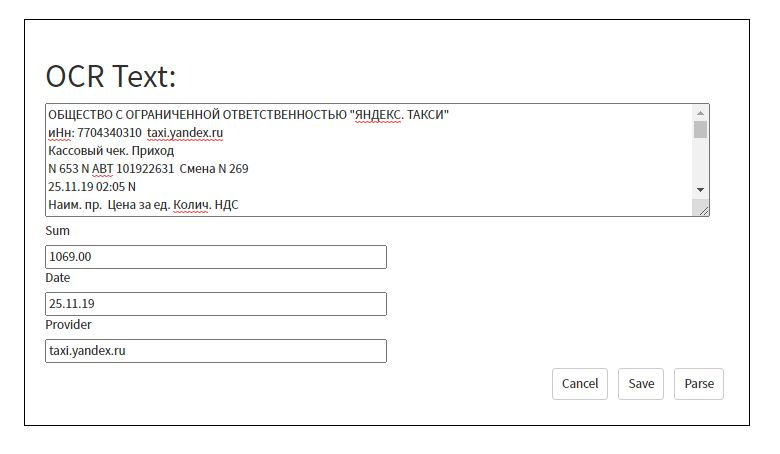
\includegraphics[scale=0.8]{Res.JPG}
  \caption{Результат работы Google Vision AI}\label{stud:fig:1234}
\end{figure}

Обратившись же к форме (рис.\,\ref{stud:fig:1235}), можно заметить, что результат, полученный c использованием библиотеки Tesseract, оказался неполным. Даже после орфографической проверки, остались неточно распознанные элементы, содержащие в себе буквы английского алфавита и другие символы. Именно поэтому поле provider осталось пустым. 
\begin{figure}[H]
  \centering
  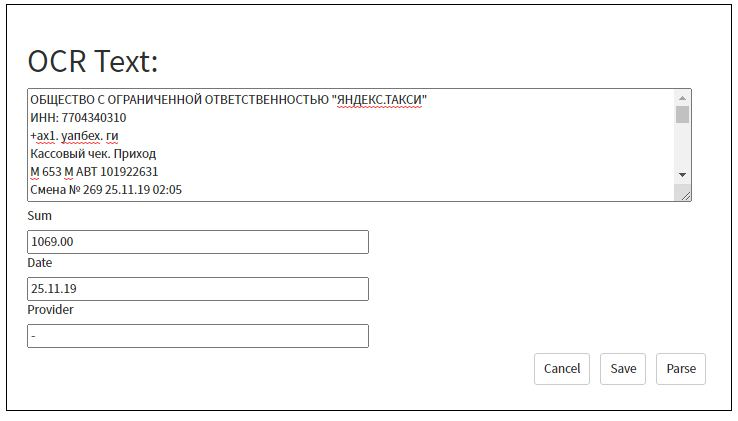
\includegraphics[scale=0.8]{Res2.JPG}
  \caption{Результат работы Tesseract.js}\label{stud:fig:1235}
\end{figure}
Из результатов тестирования можно сделать следующий выводы:
\begin{itemize}
\item Сервис Google Vision AI показал лучший результат в сравнении с Tesseract.JS,
\item В случае неполадок на сервере Google или проблем со связью по HHTP протоколу, всегда можно будет воспользоваться встраиваемой в платформу библиотекой Tesseract.JS, но необходимо будет вносить свои коррективы, чтобы качество текста оставалось на высоком уровне,
\item С помощью внедрения OCR инструментов удалось успешно автоматизировать часть процессов документооборота, отвечающих за получение данных о совершённых сотрудниками компании покупок товаров и услуг.
\end{itemize}

%=======================
\newpage
\addcontentsline{toc}{section}{Заключение}
\section*{Заключение}
В рамках данной выпускной квалификационной работе были успешно выполнены шаги по изучению базового функционала и особенностей корпоративной системы ServiceNow и методов интеграции сторонних веб сервисов в неё. Также дополнительно был проведён сбор и анализ тестовых данных, изучены принципы работы REST архитектуры. 

Результатом данного исследования являются внедрённые в платформу инструменты для распознавания текста на изображениях кассовых чеков. Использование нескольких ресурсов (Google Vision AI, Tesseract.\-JS.) стало гарантом стабильной работы приложения: в случае неполадок на сервере Google Vision AI, всегда есть возможность переключиться на Tesseract.\-JS.

В ходе данной работы получены следующие результаты: 
\begin{itemize}
\item Определён набор инструментов, успешно справляющихся с поставленной задачей,
\item Создана тестовая база, содержащая в себе кассовые чеки разных типов,
\item Настроена интеграция с библиотекой Tesseract.js и с Google Vision AI,
\item Создано модальное окно, в котором происходит пост-обработка текста,
\item Протестирован функционал инструментов,
\item Предусмотрены и исключены нежелательные сценарии.
\end{itemize}
%=======================
\newpage

\addcontentsline{toc}{section}{Литература}
\renewcommand{\refname}{\centering \textbf{Литература}}

\begin{thebibliography}{0}
\bibitem{stud:b021}
ServiceNow официальный сайт – URL: \\https://www.servicenow.com/

\bibitem{stud:b02}
Google Vision AI API – URL: \\https://cloud.google.com/vision

\bibitem{stud:b01}
Tesseract.JS библиотека – URL: \\https://unpkg.com/tesseract.js@v2.0.0-alpha.13/dist/tesseract.min.js.

\bibitem{stud:b012}
Spell-checker.js библиотека – URL: \\https://www.npmjs.com/package/spell-checker-js

\bibitem{stud:b1}
Business Rules официальная документация SN  – URL: \\https://docs.servicenow.com/bundle/orlando-application-development/\\page/script/business-rules/concept/c\_BusinessRules.html


\bibitem{stud:b2}
Script Includes официальная документация SN  – URL: \\https://docs.servicenow.com/bundle/orlando-application-development/\\page/script/server-scripting/concept/c\_ScriptIncludes.html

\bibitem{stud:b3}
REST API официальная документация SN  – URL: \\https://docs.servicenow.com/bundle/orlando-application-development/\\page/build/applications/concept/api-rest.html

\bibitem{stud:b4}
Client Scripts официальная документация SN  – URL: \\https://docs.servicenow.com/bundle/orlando-application-development/\\page/script/client-scripts/concept/client-scripts.html

\bibitem{stud:b5}
Service Portal официальная документация SN  – URL: \\https://docs.servicenow.com/bundle/orlando-servicenow-platform/\\page/build/service-portal/concept/c\_ServicePortal.html

\bibitem{stud:b6}
UI Scripts официальная документация SN  – URL: \\https://docs.servicenow.com/bundle/orlando-application\\-development/page/script/client-scripts/\-concept/c\_UIScripts.html

\bibitem{stud:b7}
UI Pages официальная документация SN  – URL: \\https://docs.servicenow.com/bundle/orlando-application-development/\\page/script/server-scripting\\/reference/r\_UIPages.html

\bibitem{stud:b8}
Performance Analytics официальная документация SN  – URL: \\https://docs.servicenow.com/bundle/orlando-performance-analytics-and\\-reporting/page/use/performance-analytics/\\reference/r\_PALandingPage.html

\bibitem{stud:b9}
System Properties официальная документация SN  – URL: \\https://docs.servicenow.com/bundle/orlando-platform-administration/\\page/administer/reference-pages/task/\\t\_AddAPropertyUsingSysPropsList.html

\bibitem{stud:b10}
UI Action официальная документация SN  – URL: \\https://docs.servicenow.com/bundle/orlando-platform-administration/\\page/administer/list-administration/\\concept/c\_UIActions.html





\bibitem{stud:b03}
Tesseract.JS репозиторий – URL: \\https://github.com/naptha/tesseract.js





\end{thebibliography}



\end{document}
% ----------------------------------------------------------------




\renewcommand\NAT@bibsetnum[1]{\settowidth\labelwidth{\@biblabel{#1}}%
   \setlength{\leftmargin}{\bibindent}\addtolength{\leftmargin}{\dimexpr\labelwidth+\labelsep\relax}%
   \setlength{\itemindent}{-\bibindent+\fivecharsapprox}%
   \setlength{\listparindent}{\itemindent}
\setlength{\itemsep}{\bibsep}\setlength{\parsep}{\z@}%
   \ifNAT@openbib
     \addtolength{\leftmargin}{\bibindent}%
     \setlength{\itemindent}{-\bibindent}%
     \setlength{\listparindent}{\itemindent}%
     \setlength{\parsep}{0pt}%
   \fi
}
\renewcommand{\thesection}{\arabic{section}.}
\renewcommand{\thesubsection}{\arabic{section}.\arabic{subsection}.}





